\documentclass[12pt]{article}
\usepackage{verbatimbox}
\usepackage{lipsum}
\usepackage{shortvrb} 
 \usepackage[T1]{fontenc}
\usepackage[utf8]{inputenc}
\usepackage{pmboxdraw}
\usepackage{newunicodechar}

\usepackage[hidelinks]{hyperref}
\usepackage[margin=1.1in ,left = 1.20in ,includefoot]{geometry}
\usepackage{graphicx}
\usepackage{float}
\usepackage[]{algorithm2e}
\usepackage{epstopdf}
\usepackage[toc,page]{appendix} 
\usepackage{amsmath}
\usepackage{fancyhdr}
\usepackage{moreverb}
\pagestyle{fancy}

%\pagestyle{headings}
\rhead{}

\usepackage{enumitem}
\usepackage{gensymb}
\usepackage{nth}
 \usepackage{hyperref}
\usepackage{subfig}
\usepackage[hidelinks]{hyperref}
\setlength{\footskip}{.8in}





% Default fixed font does not support bold face
\DeclareFixedFont{\ttb}{T1}{txtt}{bx}{n}{12} % for bold
\DeclareFixedFont{\ttm}{T1}{txtt}{m}{n}{12}  % for normal

% Custom colors
\usepackage{color}
\definecolor{deepblue}{rgb}{0,0,0.5}
\definecolor{deepred}{rgb}{0.6,0,0}
\definecolor{deepgreen}{rgb}{0,0.5,0}

\usepackage{listings}

% Python style for highlighting
\newcommand\pythonstyle{\lstset{
language=Python,
basicstyle=\ttm,
otherkeywords={self},             % Add keywords here
keywordstyle=\ttb\color{deepblue},
emph={MyClass,__init__},          % Custom highlighting
emphstyle=\ttb\color{deepred},    % Custom highlighting style
stringstyle=\color{deepgreen},
frame=tb,                         % Any extra options here
showstringspaces=false            % 
}}


% Python environment
\lstnewenvironment{python}[1][]
{
\pythonstyle
\lstset{#1}
}
{}

% Python for external files
\newcommand\pythonexternal[2][]{{
\pythonstyle
\lstinputlisting[#1]{#2}}}

% Python for inline
\newcommand\pythoninline[1]{{\pythonstyle\lstinline!#1!}}











\begin{document}
 
\begin{titlepage}
	
\thispagestyle{empty}

\begin{center}
\large {A project report on}

\Huge{\bfseries Indoor Navigation and Localization Mobile Robot }\\[0.5cm]
\large{(Final year project)}
 \\
 Submitted in partial fulfillment of the requirement for the award of the\\
 \large {Degree of Bachelor in }\\
 
 \large{\bfseries COMPUTER AND SYSTEMS ENGINEERING }\\
 
 \vspace{1.2cm}
 \begin{figure}[H]
\centering

\includegraphics[width =.45\textwidth]{Fig/faculty.png}

\end{figure}
 \vspace{.5cm}
\end{center}
 
\hspace{1cm} {\LARGE \bfseries Submitted by}  \hspace{3.5cm} {\LARGE \bfseries Supervised by:}


\hspace{0.5cm} {\bfseries  Ahmed Abdelbadee Elsayed}\hspace{2.5cm} {\bfseries  Dr.Ahmed Mohamed Helmi }

\hspace{0.5cm} {\bfseries Ahmed Abdelbasit Mohamed} 


\hspace{0.5cm} {\bfseries  Aya Ibrahim Elsayed} 


\hspace{0.5cm} {\bfseries Nourhan Mansour Mohamed} 


\hspace{0.5cm} {\bfseries Omar Raafat Abdullatif}

 
\hspace{0.5cm} {\bfseries  Yasmin Ahmed Abdelbasit}

 


\begin{center}
\today \\
 
 {\Large  \bfseries   Faculty of Engineering }\\
 
{\LARGE \bfseries Zagazig University } 
\end{center}



% Bottom of the page
 
 
 
 
 
 
 

\renewcommand{\headrulewidth}{0pt}

\end {titlepage}












\pagenumbering{roman}
\section*{\begin{center}
Abstract
\end{center}}

	This project introduces a small-size mobile robot to be used for indoor navigation. It can be operated either autonomously or controlled by man remotely over the network. Its size make it able to navigate in small places and narrow paths man can not go through.\\
	Man can discover the environment around it via a video stream transmitted by a camera free to rotate right, left, up and down. A user-friendly controller box is provided for manned control to guide robot's motion, set camera orientation and switch on/off flash light.\\
	The autonomous navigation is based on graph theory and artificial intelligence search algorithms in a predefined map for the environment around robot. With the help of Landmarks detection by computer vision, the robot can identify its location periodically on his path from source to destination. This provides a great help to avoid accumulated errors caused by hardware or sensors in accuracy.\\
	A computer graphical user interface (GUI) application is developed to easily reach the functionality of robot. By this application one can select either autonomous or manual mode and deal with each mode utilities.\\
	The project is based on Robots Operating System (ROS) which makes its functionality reusable in other projects. Modularity and readable codes are considered in the design and implementation of software nodes. Also an optimized communication protocol is developed among project's parts.\\
	About future work there is a wide field of updates like object detection, On-line Mapping of new Environments and installation of manipulator (i.e. robot arm) for a variety of	tasks.

 
\addcontentsline{toc}{section}{\numberline{}Abstract}











\newpage
\renewcommand{\headrulewidth}{0pt}
\section*{\begin{Large}
Key abbreviations
\end{Large}}

 \begin{tabular}{  l    l   }
    ROS & Robots Operating System	\\
    GUI & Graphical User Interface	\\
    RPi &   Raspberry Pi	\\
    
    PID & Proportion Integral Derivative  \\  
    PWM &  Pulse Width Modulation  \\   
    $I^2C$  & Inter-Integrated Circuit   \\  
    IMU &  Inertial Measurement Unit \\  
    LiPo &   Lithium Polymer\\ 
    RPM   & Revolution Per Minute  \\
    ADC   & Analog-Digital Converter   \\  
    LPF & Low Path Filter \\
    FPS & Frame Per Seconds\\
    GND & Ground
    
  \end{tabular} 

\addcontentsline{toc}{section}{\numberline{}Key abbreviations}
\newpage
\renewcommand{\headrulewidth}{.5pt}


\tableofcontents
\newpage
\listoffigures
\thispagestyle{empty}
\newpage
\pagenumbering{arabic}
\setcounter{page}{1}


\section{Introduction}
 In daily life there are a lot of situations in which robots are needed to perform some tasks man can not deal with. Some of these situations may be risky, difficult or such impossible for man to do. Think about a risky place we want to discover like disasters area, places of extreme environmental conditions or military purposes. In these situations introducing a robot is important for saving human life.\\
 Robots also can help people of special needs with what they can not do like carrying heavy things, holding and placing parts or even home cleaning.\\
 Robots have many configurations, styles and mechanisms for motion. Some are legged, others are wheeled and the rest can fly, swim or dive. Each configuration has its functionality that others can not do and also has limitations.
 In our project we introduce a robot with good navigation and localization technique to solve a lot of problems mentioned above in this section. 

\begin{figure}[h]
\centering
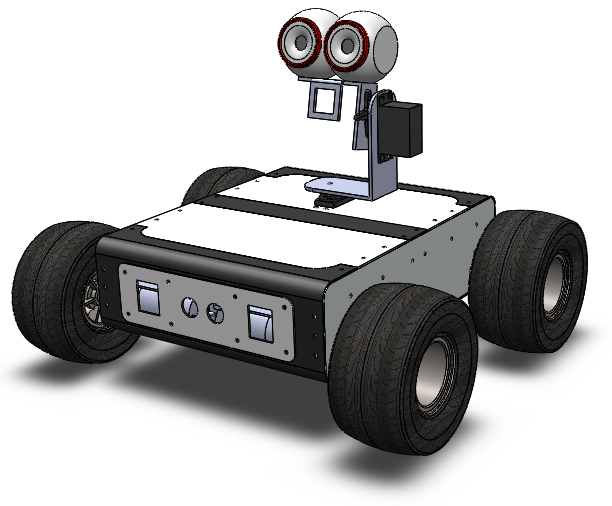
\includegraphics[width =.4\textwidth]{Fig/Introduction.png}
\caption{ A 3-D model for robot frame}
\end{figure}

%\clearpage

\subsection{History of Mobile Robots} 
Mobile robots have the capability to move around in their environment and are not fixed to one physical location. Mobile robots can be "autonomous" (AMR - autonomous mobile robot) which means they are capable of navigating an uncontrolled environment without the need for physical or electro-mechanical guidance devices. Alternatively, mobile robots can rely on guidance devices that allow them to travel a pre-defined navigation route in relatively controlled space (AGV - autonomous guided vehicle). By contrast, industrial robots are usually more-or-less stationary, consisting of a jointed arm (multi-linked manipulator) and gripper assembly (or end effector), attached to a fixed surface.\\
Mobile robots have become more commonplace in commercial and industrial settings. Hospitals have been using autonomous mobile robots to move materials for many years. Warehouses have installed mobile robotic systems to efficiently move materials from stocking shelves to order fulfillment zones. Mobile robots are also a major focus of current research and almost every major university has one or more labs that focus on mobile robot research. Mobile robots are also found in industrial, military and security settings. Domestic robots are consumer products, including entertainment robots and those that perform certain household tasks such as vacuuming or gardening. \cite{201}


\begin{figure}[H]
 \centering
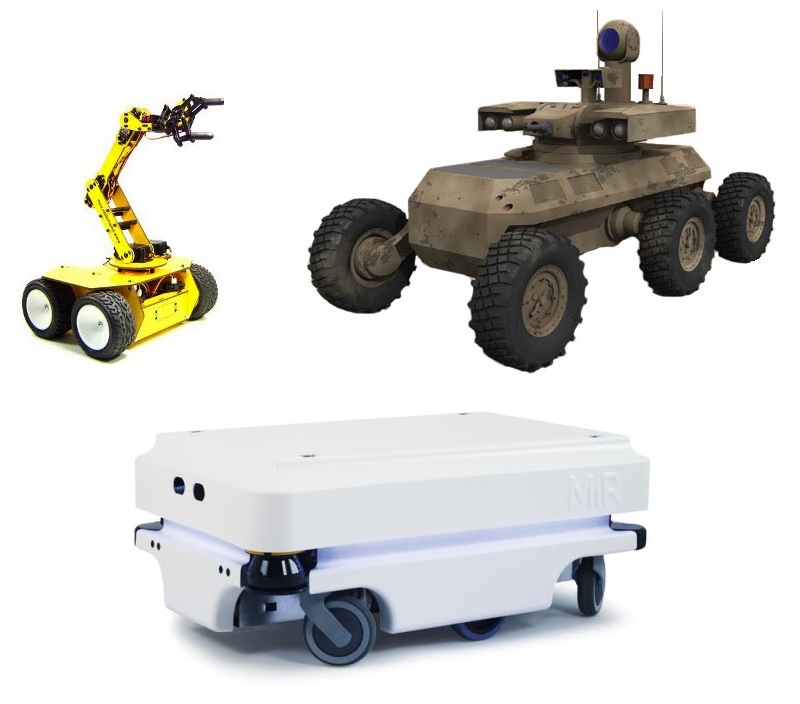
\includegraphics[width =0.6\textwidth]{Fig/mobile_robots_apps.jpg}
\caption{Different applications for mobile robots; industrial, military and transport}

\end{figure}

\subsection{Project Objectives}
The main objective of this project is to demonstrate a robust mobile robot in a small scale to perform an autonomous navigation from point to another. Also it is required for the robot to localize itself when asked to do. Both navigation and localization depends on the ability of robot to detect and recognize texts on landmarks that uniquely identifies specific nodes in the map.
For new environments whose map is not known, the robot can be guided remotely over the network to explore that location and a camera is provided for both steaming live video for the site around robot and to perform the computer vision task.
In the hardware level a robust controller is required to perform motion instructions with acceptable precision.

\newpage

\subsection{Limitations}
During our work we faced a lot of problems associated mostly with sensors. As we the main part in any control system is the feedback. This is because if we got a wrong indication for current state of system, we will perform a wrong reaction and the error increases more and more. In our project we need sensors to get information about the robot like position, velocity and orientation. Any missing part of them leads to both wrong estimation of state and wrong controller action.
In next sections we will talk about our trials, results and algorithms implemented to get the advantage of each sensor and avoid its misleading data.
\noindent But lets start from a high-level point of view and gradually take important topics with some details.

\subsection{Overview on the project parts}
The main system structure of our project as shown in following figure consists of a GUI and controller box at user side and the master unit (RPi) at robot side. The operation starts from GUI to select the function needed and then a flow of communication commands are passed to master unit over the network to perform the required task. Controller box is used in manned mode of operation to guide robot motion and camera orientation. In next chapter we talk about the GUI; how you can use, how it is implemented and a quick over view on ROS (Robots Operating System).
\begin{figure}[H]
	\centering
	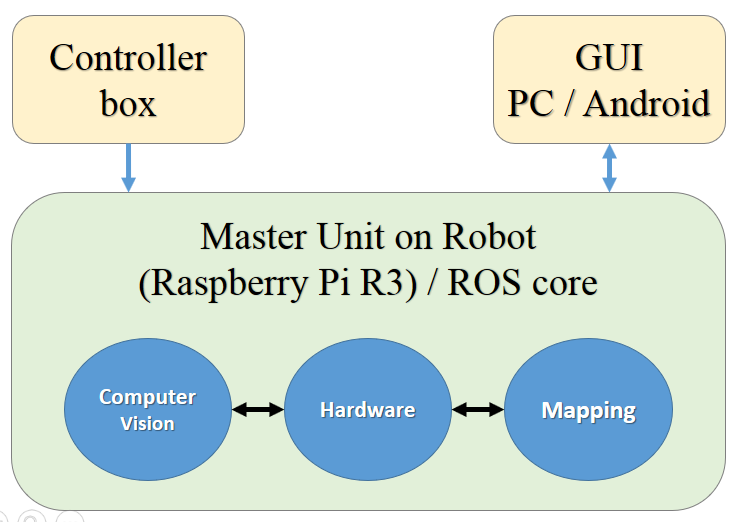
\includegraphics[width =0.6\textwidth]{Fig/overview.png}
	\caption{Clustered view of main system structure}
	
\end{figure}
\newpage

\section{User Manual and GUI}
talk about how to use the GUI to run the project on different modes.

\section{System Structure and Proposed Algorithm}
talk briefly about ROS. details of parts and communication between them. flow chart for overall processes.

\section{GUI Implementation}
talk about the Java application and how it is implemented, how it communicates with master unit. how video stream is received

\section{Mapping of Environment}
talk about graph theory and how map is represented. how landmarks are included in the map. Search algorithms. instructions created to be sent to hardware.

\section{Computer Vision}
talk about how detection, recognition and tuning are processed.

\section{Hardware Node and Low-Level Control}
mechanical analysis, solid design, final assembly, Motors choice.
Electric components, circuits, structure.
Sensors
Control system for straight line and rotation motion.

\newpage
\appendix

\section{Solid Design Parts}


\newpage
 
\bibliographystyle{abbrv}
\bibliography{final}

\end{document}

